\section{Experiments}
We assess the performance of PSRs and different kinds of Multi-PSRs on labyrinth environments. We look to see how performance varies as different parameters are varied. Parameters include the model size, the number of observations used, and the type of environment. 

\subsection{Obtaining observation sequences}
In all the experiments we consider, an agent is positioned in a starting location and it stochastically navigates the environment based on transition probabilities between states. Every time state-to-state transitions occur one observation symbol is produced. When the agent exits the labyrinth, we say the trajectory is finished, and we record the concatenation of the symbols produced. We call this concatenation an observation sequence.

MOVE THE CRAP BELOW!

In both cases, we analyse the performance for M-PSRs of different model sizes with a fixed observation data set. For each Base System M-PSR, we set $\Sigma'$ to be {$\sigma^{2^k}, k<=256 $}. For the Data-Driven PSRs we learn 10 operators from the observations with the greedy learning algorithm for obtaining $\kappa$ described in (). For all the M-PSRs, we assign $\kappa$ to the dynamic programming algorithm given in (). 

\subsection{Learning Implementation: Timing v.s Multiple Symbols}

For the timing case, we construct our empirical hankel matrix by including $\{\sigma^i, \forall i<=n\}$. With this choice, the empirical hankel matrix will be a nxn matrix with the prefixes and suffixes being the same.The parameter n depends on the application. For Double Loop environments we set n to be 300, while for pacman n was set to 600. 

For multiple observations a slightly more complex approach is required to construct the empirical hankel matrix. For prefixes P, we select the k most frequent prefixes from our observations set. For suffixes S, we take all suffixes that occur from our set of prefixes. We also require prefix completeness. That is if p' is a prefix of p $\in P$, then p' $\in P$. This heuristic for constructing empirical hankel matrices was given in previous work by [] and it showed that ().

The important property that needs to be satisfied when choosing the parameter n is that enough observations are captured to learn a good model. Something here: $\lim_{ \to 2} f(x) = 5$ .

\subsection{Measuring Performance}
For timing, the goal is to make predictions about how long the agent will survive the environment. One can also ask conditional queries such as how long the agent should expect to survive given that t seconds have elapsed $f(\sigma^m|\sigma^n) = (eqns)$. 

The goal for the multiple observation labyrinths is to make predictions about seeing observation sequences. Conditional queries are also possible here $f(a^{m_1}b^{m_2}|a^{n_1}b^{n_2}) = (eqns)$.

//DOUBLE CHECK THE ABOVE.

To measure the performance of a PSR/M-PSR we use the following norm:
$||f - \hat{f}|| = \sqrt{\sum\nolimits_{x \in observations}(f(x) - \hat{f(x)})^2}$. We use this norm because of a bound presented by [AUTHORS], which states that (). Here the function f denotes the true probability distribution over observations and the function $\hat{f}$ denotes the function associated with the learned M-PSR/PSR. In the environments that we consider the function f is obtainable directly as we have access to the underlying HMMs.

Since the set of observations $\Sigma^*$ is infinite, we compute approximations to this error norm, by fixing a set of strings T and summing over T. For the timing case, we take T to be the $\{\sigma^k, \forall k<=n\}$, while for the multiple observation case, we take all possible strings producible from the prefixes and suffixes in our dataset. That is, for the multiple observation case $T = \{ps, \forall p \in P, \forall s \in S\}$.

\section{Double Loop Timing}

For timing, we start by considering a double loop environment. The lengths of the loops correspond to the number of states in the loop. Here the lengths correspond to the number of states there are in each loop. A trajectory begins with the agent starting at the intersection of the two loops. At the intersection, the agent has a 50 percent chance of entering either loop. At intermediate states in the loops the agent moves to the next state in the loop with probability P and remains in its current state with probability 1-P. Here, P represents the self-transition probability for internal states. Exit states are located halfway between each loop. At an exit state, the agent has a 50 percent probability of exiting the environment. 

For a fixed dataset of observations, we compare the performance of a PSR and different M-PSRs and then plot the average error over the 10 datasets.

\subsection{Size of Dataset}

Here, we vary the number of observations used in our dataset. PSRs/M-PSRs learned in Figure 4 use 100 observation sequences, while those in Figure 5 use 10000. In both cases the M-PSRs outperform the standard PSR for reduced model sizes.

\subsection{Noise: Parameter P}

Next, we vary the self-transition probability P to simulate noise in an environment. Figure 5 is a 64-16 double loop with P=0.2, and Figure 6 is a 64-16 double loop with P=0. We find that the noisy loops are more compressible, but the performance is worse for higher models. Nevertheless, M-PSRs still significantly outperform the standard PSR for reduced model sizes.

\subsection{Varying Loop Lengths}

So far we have been using a 64-16 Double Loops. Here observations will come in low multiples of large powers of two. Intuitively, in this case the Base M-PSR should shine the most. In Figure 8, we plot the results of a 47-27 labyrinth where observations will not be so easily expressed from the Base M-PSR. Once again, M-PSRs outperform the standard PSR for reduced model sizes. In addition we see that the Data-Driven M-PSR does better than the Base M-PSR.

\section{Large Labyrinth Timing}

We proceed to work with a more complex labyrinth environment. Figure 10 shows it's graphical representation. We test a larger environment as results in such a system would transfer to applications such as pacman. Transitions to new states occur with equal probability. The weight between transitions corresponds to the number of time steps. We add an additional parameter sF: stretchFactor, which multiplies all of the weights in the graph. 

\subsection{Vary data}

In Figures 11 and 12 we vary the number of observations used to learn PSRs/M-PSRs. We find that ().

\subsection{Vary StretchFactor}

In Figures 13 and 14 we vary the stretchFactor parameter. We find that ().

\section{Multiple Observations: Colored Loops}

We now move to the multiple observation case. Here the Data-Driven M-PSRs really show their strength as observation sequences are more complex. We construct a Double Loop environment where one loop is green and the other is blue. The lengths of each loop are also varied, see Figure 4 and Figure 5. We fix the length of observations to be $TrajectoryLength := (len(loop1) + len(loop2))*3$. To build empirical estimates of probabilities we set $f(x)=(pocc(x)/numstringslength>=x$. This means that the PSRs will compute the probability of a prefix occurring.

\subsection{Data dif amounts}

As for the timing case, we vary the amount of data to learn PSRS/M-PSRs in Figures 15 and 16. Once again we find ().

\subsection{Loop Lengths dif amounts}
In figures 17,18 we vary the loop lengths. When the GCD loop lengths is a high power of 2, the Base M-PSR does similar to the Data-Driven M-PSR. However, when the loop lengths are 27-17, we find that the Data-Driven M-PSR does far better. This shows that learning $\Sigma'$ from data offers a significant advantage.


\begin{figure}[ht!]
\centering
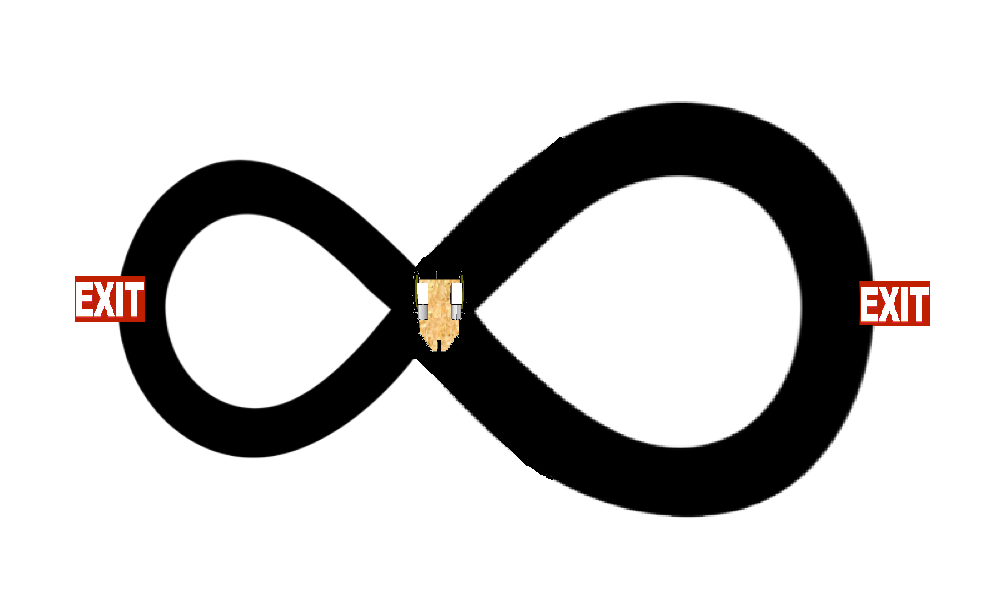
\includegraphics[width=60mm]{uCOREPICS/doubleLoopImage.png}
\caption{Double Loop Environment\label{overflow}}
\end{figure}

\begin{figure}[ht!]
\centering
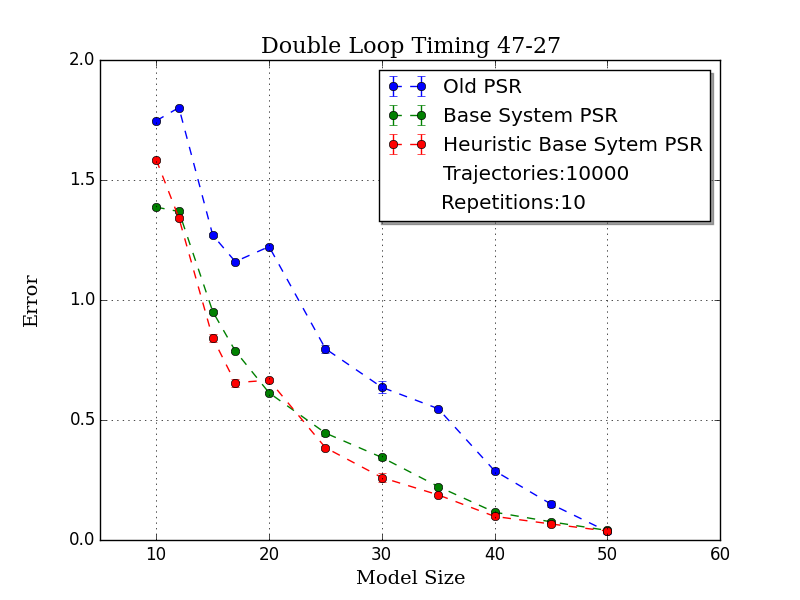
\includegraphics[width=60mm]{uCOREPICS/DoubleLoop47-27Heuristics.png}
\caption{Double Loop 47-27\label{overflow}}
\end{figure}

\begin{figure}[ht!]
\centering
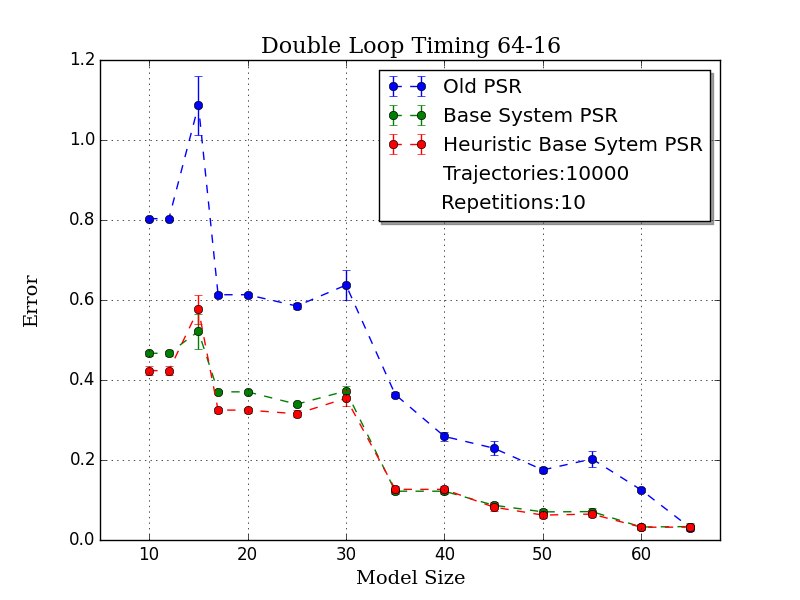
\includegraphics[width=60mm]{uCOREPICS/DoubleLoop64-16Heuristics.png}
\caption{Double Loop 64-16\label{overflow}}
\end{figure}

\begin{figure}[ht!]
\centering
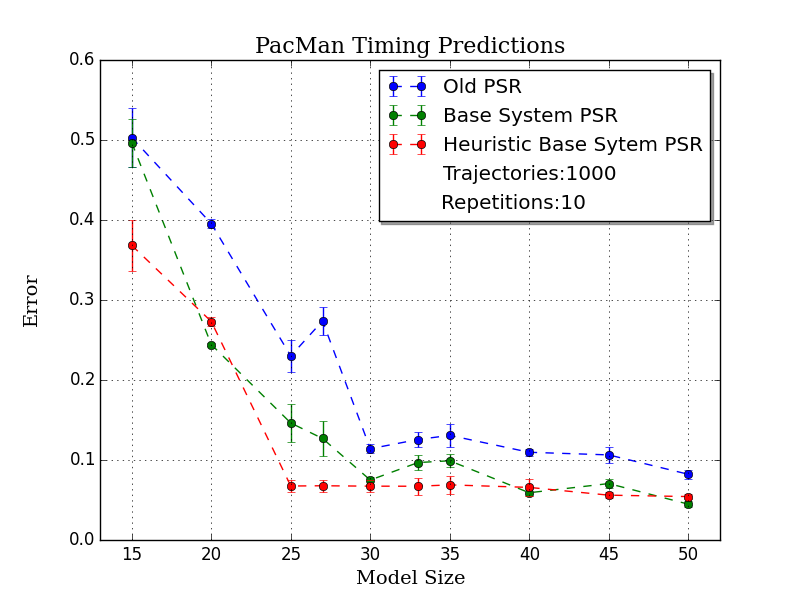
\includegraphics[width=60mm]{uCOREPICS/PacManTimingHeuristicsIncluded.png}
\caption{Pacman Labyrinth\label{overflow}}
\end{figure}

\begin{figure}[ht!]
\centering
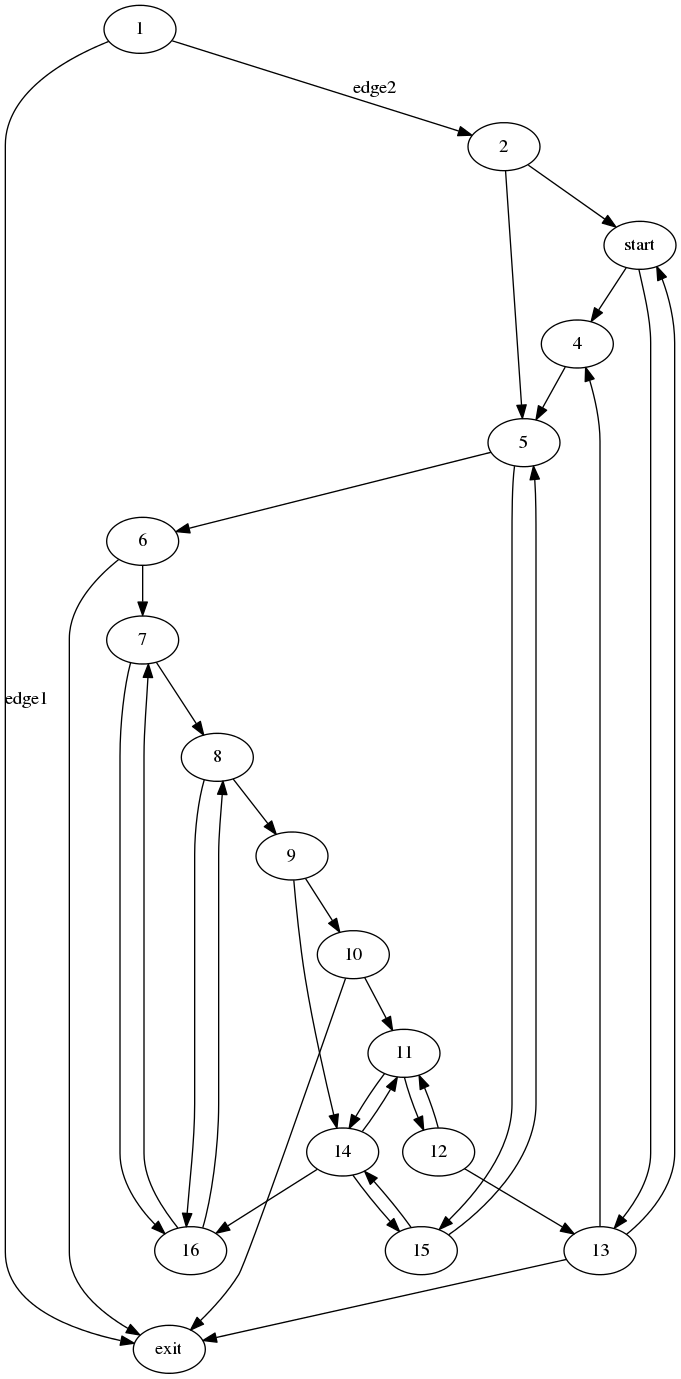
\includegraphics[width=40mm,height=60mm]{uCOREPICS/graphPacMan.png}
\caption{Graph of pacman\label{overflow}}
\end{figure}

\subsection{Experimental Data Driven Sigma'}
For the double loop case the data-driven greedy approach learns multiples of the loop lengths which results in partitions which use fewer operators. As an example, for the 47-27 labyrinth the heuristic included included the following operators: $\Sigma'=\{\sigma^{47}, \sigma^{27}, \sigma^{74}, \sigma^{94} ...\}$. For Pacman, the learned strings are multiples of the stretch factor. For Colored Double Loops, $Sigma' = \{g^{27},b^{17},g^{27}b^{17},\}$ The top 7 of 10 operators are usually learned consistently, while the other strings vary slightly dependent on the generated dataset.

\subsection{Discussion}

some discussion of results...

\begin{figure}[ht!]
\centering
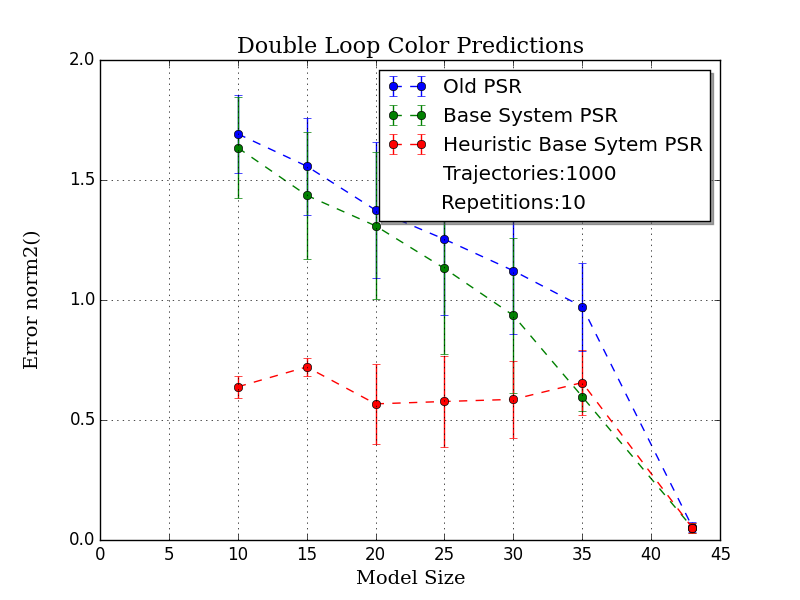
\includegraphics[width=60mm]{uCOREPICS/MultipleObservationsHeuristics.png}
\caption{Colored Loops 27-17\label{overflow}}
\end{figure}

\begin{figure}[ht!]
\centering
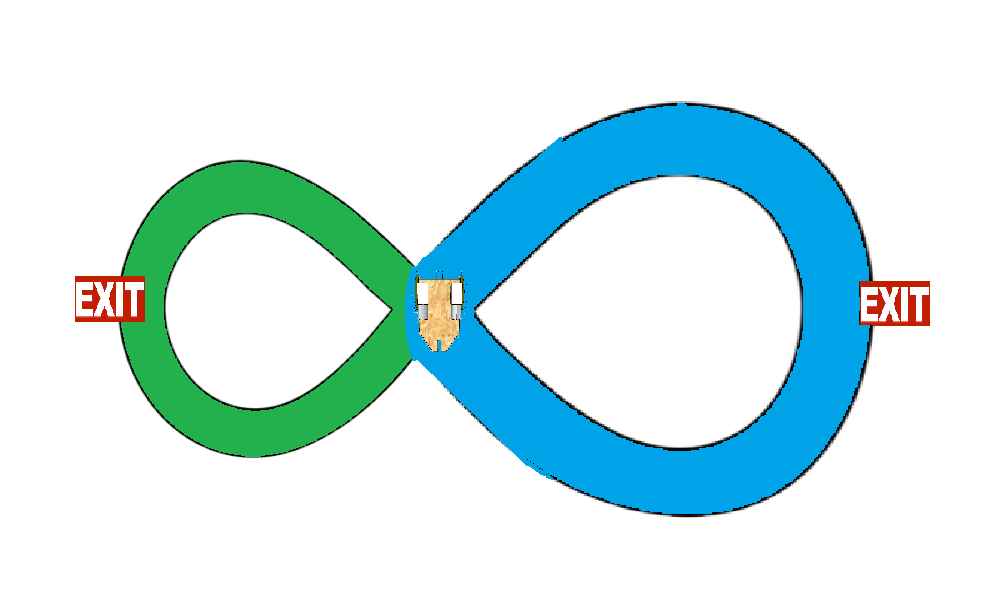
\includegraphics[width=60mm]{uCOREPICS/doubleLoopImageMO.png}
\caption{Colored Loops Environment\label{overflow}}
\end{figure}
